\documentclass{report}

\usepackage{pgfplots}
\pgfplotsset{compat=1.18}
\usepackage{tikz}
    \usetikzlibrary{arrows.meta}

\begin{document}
\section{Coordinates}
\begin{figure}[!h]
\centering
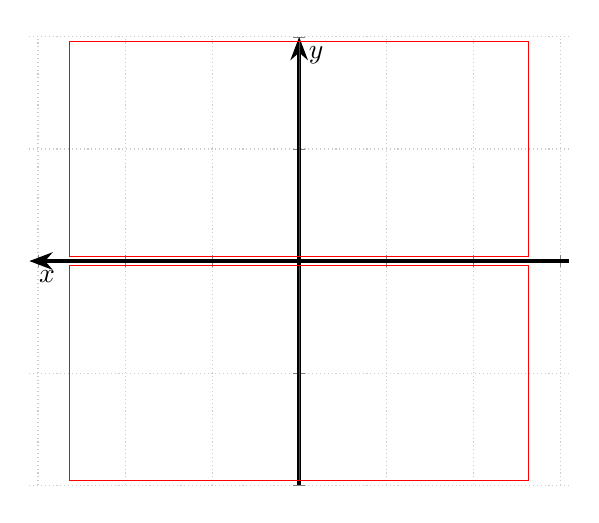
\begin{tikzpicture}
    \def\x{13.19};
    \def\y{9.8};
    \begin{axis}[
	axis lines = middle,
	axis line style = {-Stealth, very thick},
	xmin = -15.5, xmax = 15.5, ymin = -10, ymax = 10,
	x dir = reverse,
	% xtick distance = 1,
	% ytick distance = 1,
	xticklabel = \empty,
	yticklabel = \empty,
	xlabel = $x$,
	xlabel style = { at = {(current axis.left of origin)}, anchor = south west, below right},
	ylabel = $y$,
	grid = major,
	grid style = {thin, densely dotted, black!20} ]
	\draw[red] (0,  0.2) rectangle ( \x,  \y);
	\draw[red] (0,  0.2) rectangle (-\x,  \y);
	\draw[red] (0, -0.2) rectangle ( \x, -\y);
	\draw[red] (0, -0.2) rectangle (-\x, -\y);
    \end{axis}
\end{tikzpicture}
\end{figure}

\end{document}
